\documentclass[a4paper, 11pt]{article}
\usepackage{comment} % enables the use of multi-line comments (\ifx \fi) 
\usepackage{fullpage} % changes the margin
\usepackage{graphicx}
\usepackage{minted} % sudo easy_install Pygments  
\usepackage[section]{placeins}


\begin{document}
\noindent
\large\textbf{Post-Lab 2 Report} \hfill \textbf{Piotr Giedziun} 184731\\
\normalsize Secure Systems and Networks \hfill  Lab Date: 04/11/14 \\
dr inż. Tomasz Surmacz

\section*{Abstract}
This report presents implementation and analysis of network scanner. This paper describes consecutive iterations of scanning software and some basics analysis.
For a selected internal network I found several servers with outdated and insecure software installed. However, the goal of this task did not consisted of vulnerability testing. Few open SMTP servers were found, although none of the four were actually vulnerable.

\section*{Introduction}
Our task was to scan given network range and investigate found services. Investigation require us to gather detailed information about each opened service (such as version, name). Having those information we are able to determine if given software might be harmful for the server. 
In addition we were asked to run additional test for mail servers, in order to find out, if "open mail relay" were found.
An open mail relay is a name for an SMPT server configured in such a way that it allows anyone on the Internet to send e-mail through it.

\section*{Network scanning}

The lab room local network (in my case IP range 156.17.40.1-254) was scanned for all services such as SSH, SMTP, FTP, HTTP, HTTPS.
Due to the excessively long scanning time, I decided to limit the range of ports to 22-443 (range of SSH to the HTTPS).
I'm aware of the fact, that redirected ports (such as 22 $\rightarrow$ 2222) will not be found due to enforced limitation. However, in order to fit in given time I had to limit that range.

I decided to use "Network Mapper" (nmap) to scan network. It's open source software, that uses raw IP packets in novel ways to determine what hosts are available on the network, what services (application name and version) those hosts are offering, what operating systems they are running, what type of packet filters/firewalls are in use, and dozens of other characteristics.

First application (Listing \ref{lst:first_app}) supposed to list all open ports alongside with version and others available information.
Software was written in python 2.7 using nmap wrapper. It's just class wrapper for a nmap build-in package.
Another package I used was `PrettyTable`, it's a simple Python library, that allows to create ASCII tables.

Figure \ref{fig:all_server_list} shows a fragment of received data. I was looking for UDP and TCP protocols, however I didn't found single UDP instance.
Almost all services were running on default port, with only exception, which caught my attention. On machine 156.17.40.227 Apache is deployed on both ports 80 and 90. I will describe tests performed on 156.17.40.227 in next section.

\begin{listing}[!htb]    
\caption{Network Scanner - first implementation.}    
\inputminted[mathescape, fontfamily=tt, frame=leftline,framerule=0.4pt,framesep=2mm]{python}{scripts/scan_all.py}
\label{lst:first_app}    
\end{listing}

\begin{figure}[!htb]
  \centering
      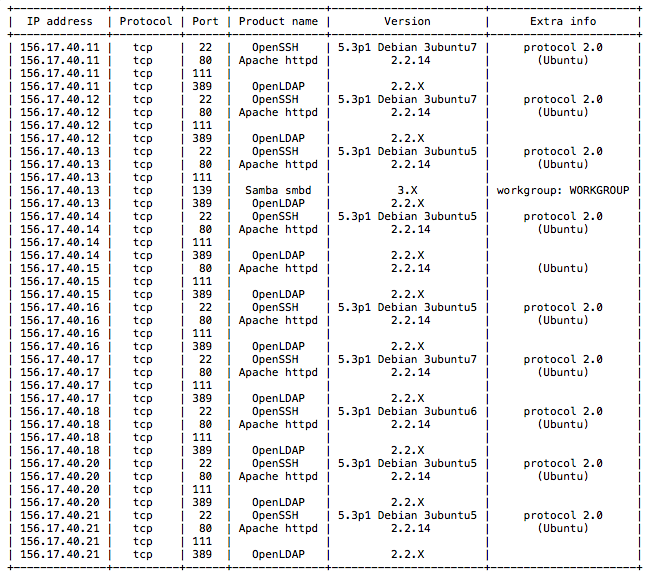
\includegraphics[width=1\textwidth]{tables/port_scan_all}
  \caption{Selected scanned IP adresses}
  \label{fig:all_server_list}    
\end{figure}


\section*{Looking for insecure software}

Another part of the laboratory was to perform manual scan of obsolete or insecure version of software installed on scanned machines.
We had all necessary informations already, therefore this part was rather simple. There are several websites thats aggregates information about specific application vulnerabilities, one of them have an API, so entire process could be automatized.

List of machines that have vulnerable software installed (in case of multiple instances running the same version of software - only one was listed)

\begin{table}[h]
  \centering
\begin{tabular}{|l|l|l|l|c|}
\hline
\multicolumn{1}{|c|}{IP Address} & \multicolumn{1}{c|}{Port} & \multicolumn{1}{c|}{Software name} & \multicolumn{1}{c|}{Software version} & CVSS Score                              \\ \hline
156.17.40.105                    & 80                        & Microsoft IIS webserver            & 7.5                                   & {\color[HTML]{FE0000} \textbf{10.0/10}} \\ \hline
156.17.40.148                    & 25                        & Exim smtpd                         & 4.72                                  & {\color[HTML]{F56B00} 7.5/10}           \\ \hline
156.17.40.12                     & 389                       & OpenLDAP                           & 2.2.X                                 & {\color[HTML]{F56B00} 7.1/10}           \\ \hline
156.17.40.220                    & 22                        & OpenSSH                            & 3.8.1p1                               & {\color[HTML]{FE0000} \textbf{9.3/10}}  \\ \hline
156.17.40.18                     & 22                        & OpenSSH                            & 5.3p1                                 & {\color[HTML]{F56B00} 7.5/10}           \\ \hline
156.17.40.85                     & 25                        & Sendmail                           & 8.14.3                                & {\color[HTML]{F56B00} 7.5/10}           \\ \hline
\end{tabular}
\end{table}


I'm not going to explain in details each security vulnerabilities, instead I will focus on few of them. Detailed description of each listed applications and their versions can be found on cvedetails.com. 

First worth describing vulnerability is ability to bypass intended access restrictions via a crafted client certificate. Sendmail version 8.14.3 is the last release with bug. That's the only major issue with Sendmail. Another bypass attack is available on Openssh version 5.3, LDAP user can be successfully authenticated without knowledge of the shared secret. Installed version of Openssh is also vulnerable to DoS attack, that  will cause memory corruption.
Last but not least, Microsoft IIS webserver with multiple flaws. IIS 7.5 allows remote attackers to execute arbitrary code or cause a denial of service.

I also did some private analysis on previously mentioned PHP script on machine 156.17.40.227 (port 90), although there is no major issue I decided to spent some time to describe it. Site is vulnerable to XSS attack, limited (not harmful) SQL Injection and other less important flaws. Another worth pointing out issue is invalid PHP configuration, when invalid arguments will be provided to the script, PHP error log will be returned (with server paths, internal file names). I did use sqlmap to find out whenever search parameter is injectable and it's vulnerable to SQL inject, although percent sign is not filtered - parameter value is injected to the query in insecure way. As presented in Figure \ref{fig:sql_inject} I did filter city name by starting with letter "B". Suppose, that the same query builder was used for authentication. We would be able to login using username=\% and password=\%.


\begin{figure}[!htb]
  \centering
      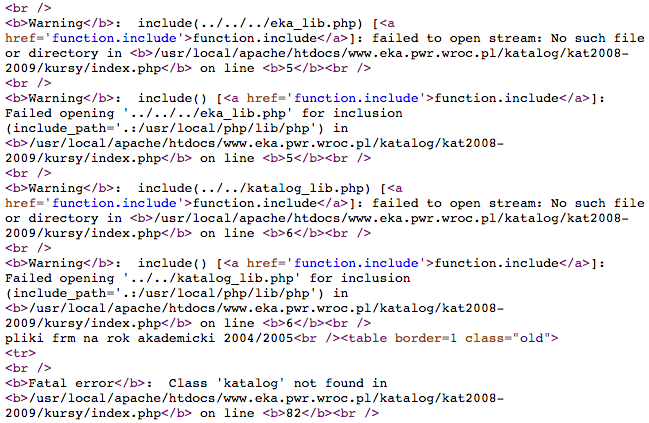
\includegraphics[width=0.8\textwidth]{apache/php_error}
  \caption{PHP configuration flaw}
  \label{fig:php_error}    
\end{figure}

\begin{figure}[!htb]
  \centering
      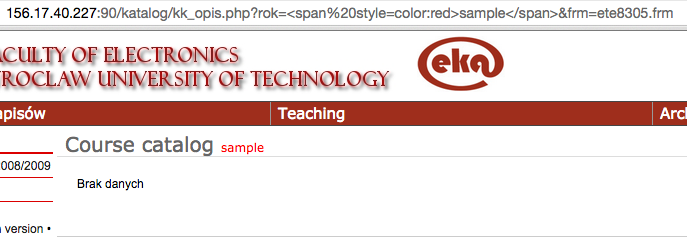
\includegraphics[width=0.8\textwidth]{apache/XSS_injection}
  \caption{XSS code injection}
  \label{fig:xss_inject}    
\end{figure}

\begin{figure}[!htb]
  \centering
      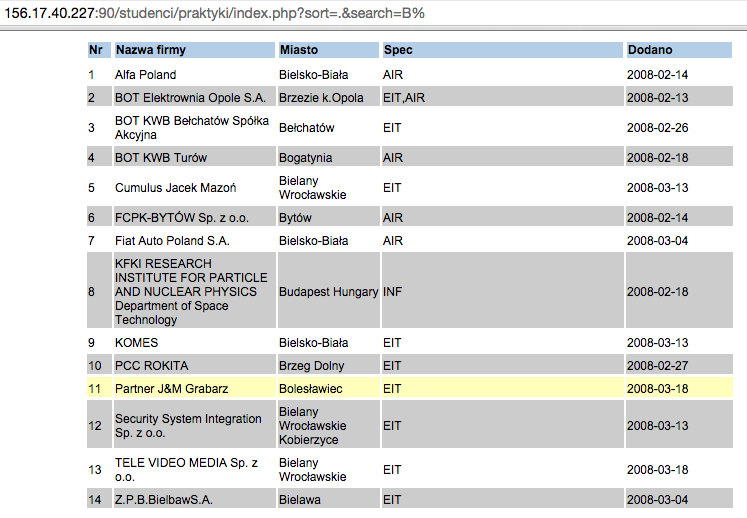
\includegraphics[width=1\textwidth]{apache/sql_inject}
  \caption{Invalid input filtering}
  \label{fig:sql_inject}    
\end{figure}

\section*{Open mail relay scan}
All previously found mail servers should be tested whether they are "closed" or "open relay". 
Following code (Listing \ref{lst:scan_mail}) was used to obtain list of servers with available SMTP.
It's slight modified version, looking only for port 25. List of found services is shown is Figure \ref{fig:mail_scan}.

\begin{listing}[!htb]    
\caption{Network Scanner - just mail services.}    
\inputminted[mathescape, fontfamily=tt, frame=leftline,framerule=0.4pt,framesep=2mm]{python}{scripts/scan_mail.py}
\label{lst:scan_mail}    
\end{listing}

Using found IP addresses of a SMTP servers we can proceed to "open relay" test. I used the data given in task description ("xx@plonk.ict.pwr.wroc.pl" and "zxcvbnm@heaven.org"). I created simple Python script, whose job is to determine whatever server is vulnerable or not.

\begin{figure}[!htb]
  \centering
      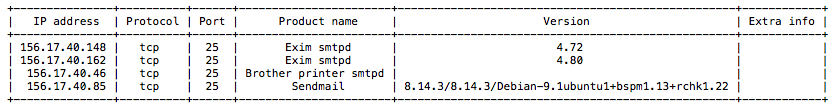
\includegraphics[width=1\textwidth]{tables/mail_scan_all}
  \caption{Mail services}
  \label{fig:mail_scan}    
\end{figure}

\begin{listing}[!htb]    
\caption{Open relay testing code}    
\inputminted[mathescape, fontfamily=tt, frame=leftline,framerule=0.4pt,framesep=2mm]{python}{scripts/check_servers.py}
\label{lst:scan_mail}    
\end{listing}

\begin{figure}[!htb]
  \centering
      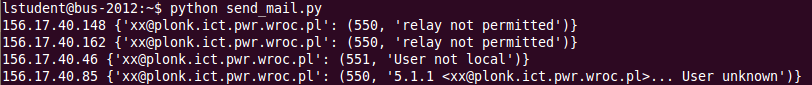
\includegraphics[width=1\textwidth]{screenshots/send_mail}
  \caption{Scanning resutl}
  \label{fig:mail_scan_result}    
\end{figure}

None of found services is vulnerable to "Open mail relay", all of them returned 55X error message (as shown in Figure \ref{fig:mail_scan_result}).


\begin{thebibliography}{9}

\bibitem{computerhope} http://www.computerhope.com/unix/nmap.htm
\bibitem{cvedetails}  http://www.cvedetails.com/
\bibitem{dream} http://dream.ict.pwr.wroc.pl/ssn/index.en.html

\end{thebibliography}

\end{document}
